\documentclass{llncs}

\usepackage{graphicx}

\title{Flexible Scientific Data Management for Plant Phenomics Research}

%Autors: Peter Ansell1, Robert Furbank2, Kutila Gunasekera1, Jianming Guo2,
%David Benn3, Gareth Williams3, Xavier Sirault2
\author{Peter Ansell\inst{1}, Robert Furbank\inst{2}, Kutila Gunasekera\inst{1},
Jianming Guo\inst{2}, David Benn\inst{3}, Gareth Williams\inst{3}, Xavier
Sirault\inst{2}}

%Affiliation:
\institute{
      eResearch Group, School of Information Technology and Electronic
Engineering,
             University of Queensland, Brisbane, Australia
 \and CSIRO Plant industry, High Resolution Plant Phenomics Centre, Canberra,
Australia
 \and CSIRO IM\&T Advanced Scientific Computing and Research Data Services,
Melbourne, Australia}
 
\begin{document}

\maketitle

\begin{abstract}
 
In this paper, we expand on the design and implementation of the Phenomics
Ontology Driven Data repository \cite{Li2010} (PODD) with respect to the
capture, storage
and retrieval of data and metadata generated at the High Resolution Plant
Phenomics Centre (Canberra, Australia). PODD is a schema-driven Semantic Web
database which uses the Resource Description Framework (RDF) model to store
semi-structured information. RDF allows PODD to process information about a
range of phenomics experiments without needing to define a universal schema for
all of the different structures. To illustrate the process, exemplar datasets
were generated using a medium throughput, high resolution, three-dimensional
digitisation system purposely built for studying plant structure and function
simultaneously under specific environmental conditions. The High Performance
Compute (HPC), storage and data collection publication aspects of the workflow
and their realisation in CSIRO infrastructure are also discussed along with
their relationship to PODD.

\end{abstract}

\keywords{eResearch, Semantic Web, RDF, OWL, Data collection citation, BagIt, Data Access Portal}

\section{Introduction}
Since the genomics era, biology has become a data-driven science. Advances in
robotics, automation and imaging, in combination with high performance computing
have permitted the rapid production of large and complex biological datasets.
Currently, high volumes of heterogeneous image data, physiological and
morphological measurements are being acquired by a range of new phenotyping
platforms located in purpose built phenomics centres across the world. These
large datasets of phenotypic characteristics such as growth rate, plant architecture,
photosynthetic performance, yield must be stored and correlated with genotypes. These factors provide evidence of genetic variation in natural and derived genetic populations (e.g. germplasm collections, association genetic panels, recombinant inbred lines). They also enable a deeper understanding the dynamic relationship between phenotype, genotype and environment which is necessary to continue delivering the increase in productivity necessary for feeding the world.


The vast array of phenotypic data collected from a variety
of phenomics platforms must be combined with metadata explaining how the raw
data was collected. This combination of raw data and metadata are then delivered to a range of analysis pipelines, which transform the raw data into aggregated
multi-phase datasets, each phase representing a new aggregation or inference
from the original raw data. This reduction process converts the raw
multi-dimensional data into information which is conceptually interpretable by a
human being, i.e. new knowledge. The additional metadata describing the steps taken are recorded to give context to the data. 
% These links enable scientists to generate novel
% conclusions about the plants being phenotyped, including conclusions based on
% the genotype, plant growth environments, treatments, phenotyping platforms and
% the phenotyping and analysis processes.


To make sense of this large amount of information, sophisticated storage,
archiving, searching and analysis capabilities are required. To date solutions
to this problem have been handled essentially by private companies, and no
suitable solution exists in the public domain. Lack of systems, both to manage
linked metadata, and controlled vocabularies to describe plant growth and
experimental conditions, have severely hampered sharing of plant phenomics data,
comparison of results between laboratories and the capacity to carry out
meta-analysis of existing data sets.


Thus, to support publicly-funded phenomics activities in Australia, the
Phenomics Ontology Driven Data repository (PODD) has been developed as a
repository for data produced by the variety of plant imaging and phenotyping
platforms available at the High Resolution Plant Phenomics Centre, as well as
for recording the contextual metadata associated with plant genotypes,
treatments and environmental conditions \cite{Li2010}. 
% PODD manages the links between the
% raw image files generated by plant imaging platforms, the results from analyses,
% and conclusions by scientists.


In this paper, we describe the workflow management that the High Resolution
Plant Phenomics Centre (HRPPC) has implemented for keeping track of its
phenomics data, metadata and experimental processes. This complex challenge was
addressed by building a multi-disciplinary group of information technology
experts and embedding users of phenomics technologies into it. The result of the
approach is a state of the art computational and data mining environment,
optimised for data access, data discovery and data sharing, which also provides
the flexibility for linking genomic information through the use of RDF triples.
In this context, we also describe the role of the CSIRO Data Access Portal (DAP) \cite{DAP}
%http://data.csiro.au) 
to annotate and store raw and processed datasets. DAP also
provides long term secure storage for data collections and the ability to search
for, control access to, and cite them via Digital Object Identifiers. PODD
manages the mapping of collections located in DAP to PODD projects, providing
for the storage of large images and documents unsuited to RDF databases. Figure~\ref{hrppccomponents} 
shows the relationship between components and key data flows.


%%Figure 1. HRPPC component relationships and data flow
\begin{figure}
\begin{center}
 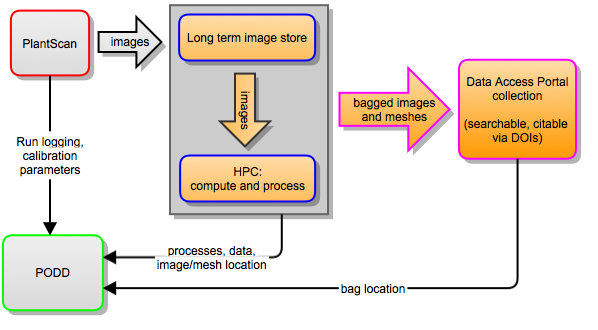
\includegraphics[width=12cm,keepaspectratio=true]{plantscan-workflow-figure1.png}
 % plantscan-workflow-figure1.png: 598x330 pixel, 72dpi, 21.10x11.64 cm, bb=0 0
%598 330

\caption{HRPPC component relationships and data flow}
\label{hrppccomponents}
\end{center}
\end{figure}


\section{Phenomics Ontology Driven Data repository}
\subsection{Semantic science for phenomics data management}
Scientists have focused on including semantics into datasets, typically using
the foundations of RDF and OWL, from two main directions. Some focus on defining
ontologies based on hierarchies of scientific concepts and properties, while
others have focused on mapping complex scientific datasets to RDF using syntax
transformations without initially defining the semantic meaning of the results.
In reality, most efforts fall somewhere in the middle, with ontological
annotations attached to some data points while other nearby data points are
syntactically represented using RDF, without links to ontologies of scientific
concepts.


Increasingly however, providers of scientific datasets are focusing on enhancing
their datasets using curated scientific concepts from ontologies. For example,
scientists have used the Gene Ontology \cite{Ashburner2000} to link well known concepts to
represent common elements across genomics datasets, while the Plant Ontology \cite{Avraham2008} 
allows the description of plant based datasets. 
% If these annotations are
% given using recognised URIs, and not as key-value string tuples, various RDF
% documents can be merged automatically based on RDF semantics to discover novel
% conclusions. 
% Initially, different providers were not able to decide on URIs to
% use in Linked Data. This resulted in various third parties such as Bio2RDF
% \cite{Belleau2008}
% creating RDF versions of scientific datasets so that the RDF documents could be
% easily merged based on common URIs. However, recently more providers have given
% authoritative URIs for each object in their dataset, making it easy to integrate
% data from various locations.


\subsection{Redesign of the Phenomics Ontology Driven Data repository}
The PODD repository relies on semantic web technologies to
manage phenomics data and metadata. Although both ontologies and mappings are
essential, in PODD it was necessary to build the system with a relaxed
ontological vocabulary to allow scientists to generate datasets before they were
certain about the semantic meaning of their work. In addition, it was necessary
for PODD to allow scientists to continue to maintain projects containing curated
scientific concepts alongside raw experimental data. The PODD repository was 
redesigned based on an evaluation of the original software \cite{Li2010} that 
found it was not able to scale sufficiently to suit the HRPPC needs. The 
major differences to the software implemented by \cite{Li2010} are that projects 
are no longer the only supported top object type, and projects are not stored 
in multiple parts, as that approach was not able to scale as was originally hypothesised.


The basic PODD project is structured as a tree, which, when used with
PlantScan\textsuperscript{\texttrademark}, represents the different components
of a scientific project as
top-level branches. These include a branch for raw data, along with separate
branches for results, analysis, and publications related to the project. In the
case of raw data, the semantics are not clear and cannot be defined by the
platforms collecting the data. 
% Scientists are able to sparsely attach meaning
% using horizontal links between different branches, using the OWL Open World
% Assumption to allow extra semantic annotations to be attached in future. 
For example, they may annotate images of a plant with a trait in only one case,
without annotating other images. These horizontal links are not constrained by
the basic scientific project structure, so they are able to entail novel
meanings independent of the ontology, including untested hypotheses, process
annotations and meaningful scientific results.


\subsection{Semantic validation}
PODD validates experiments using independently configurable rules based on OWL
(Web Ontology Language) schemas. Although PODD currently only supports OWL as a
rules language, it could be easily extended in other cases to use different
systems such as N3, RDFS, SPARQL, or SPIN as rules languages \cite{Fuerber2010}. 


OWL is used to determine whether projects are both internally consistent, with
all objects having an explicit RDF type, and whether they are consistent with
the ontologies that they import. The main point that PODD focuses on for
validation is determining that mappings are consistent with the basic PODD
predicates and classes, so that they can be used to render both static HTML
pages and provide HTML based editing facilities. For example, any OWL object
property that has been defined to link from image acquisition runs to images can
be used to define the purpose of an image. This may include any combination of
the defined properties, without requiring all of the properties to be used.
% The parent object types and properties used by PODD to establish basic ground
% rules for rendering and validation are defined in a small base schema ontology.
General scientific properties and phenotype specific properties are defined
in larger extension ontologies as illustrated in Figure~\ref{poddontologies}.

%Figure 2. 
\begin{figure}
\begin{center}
 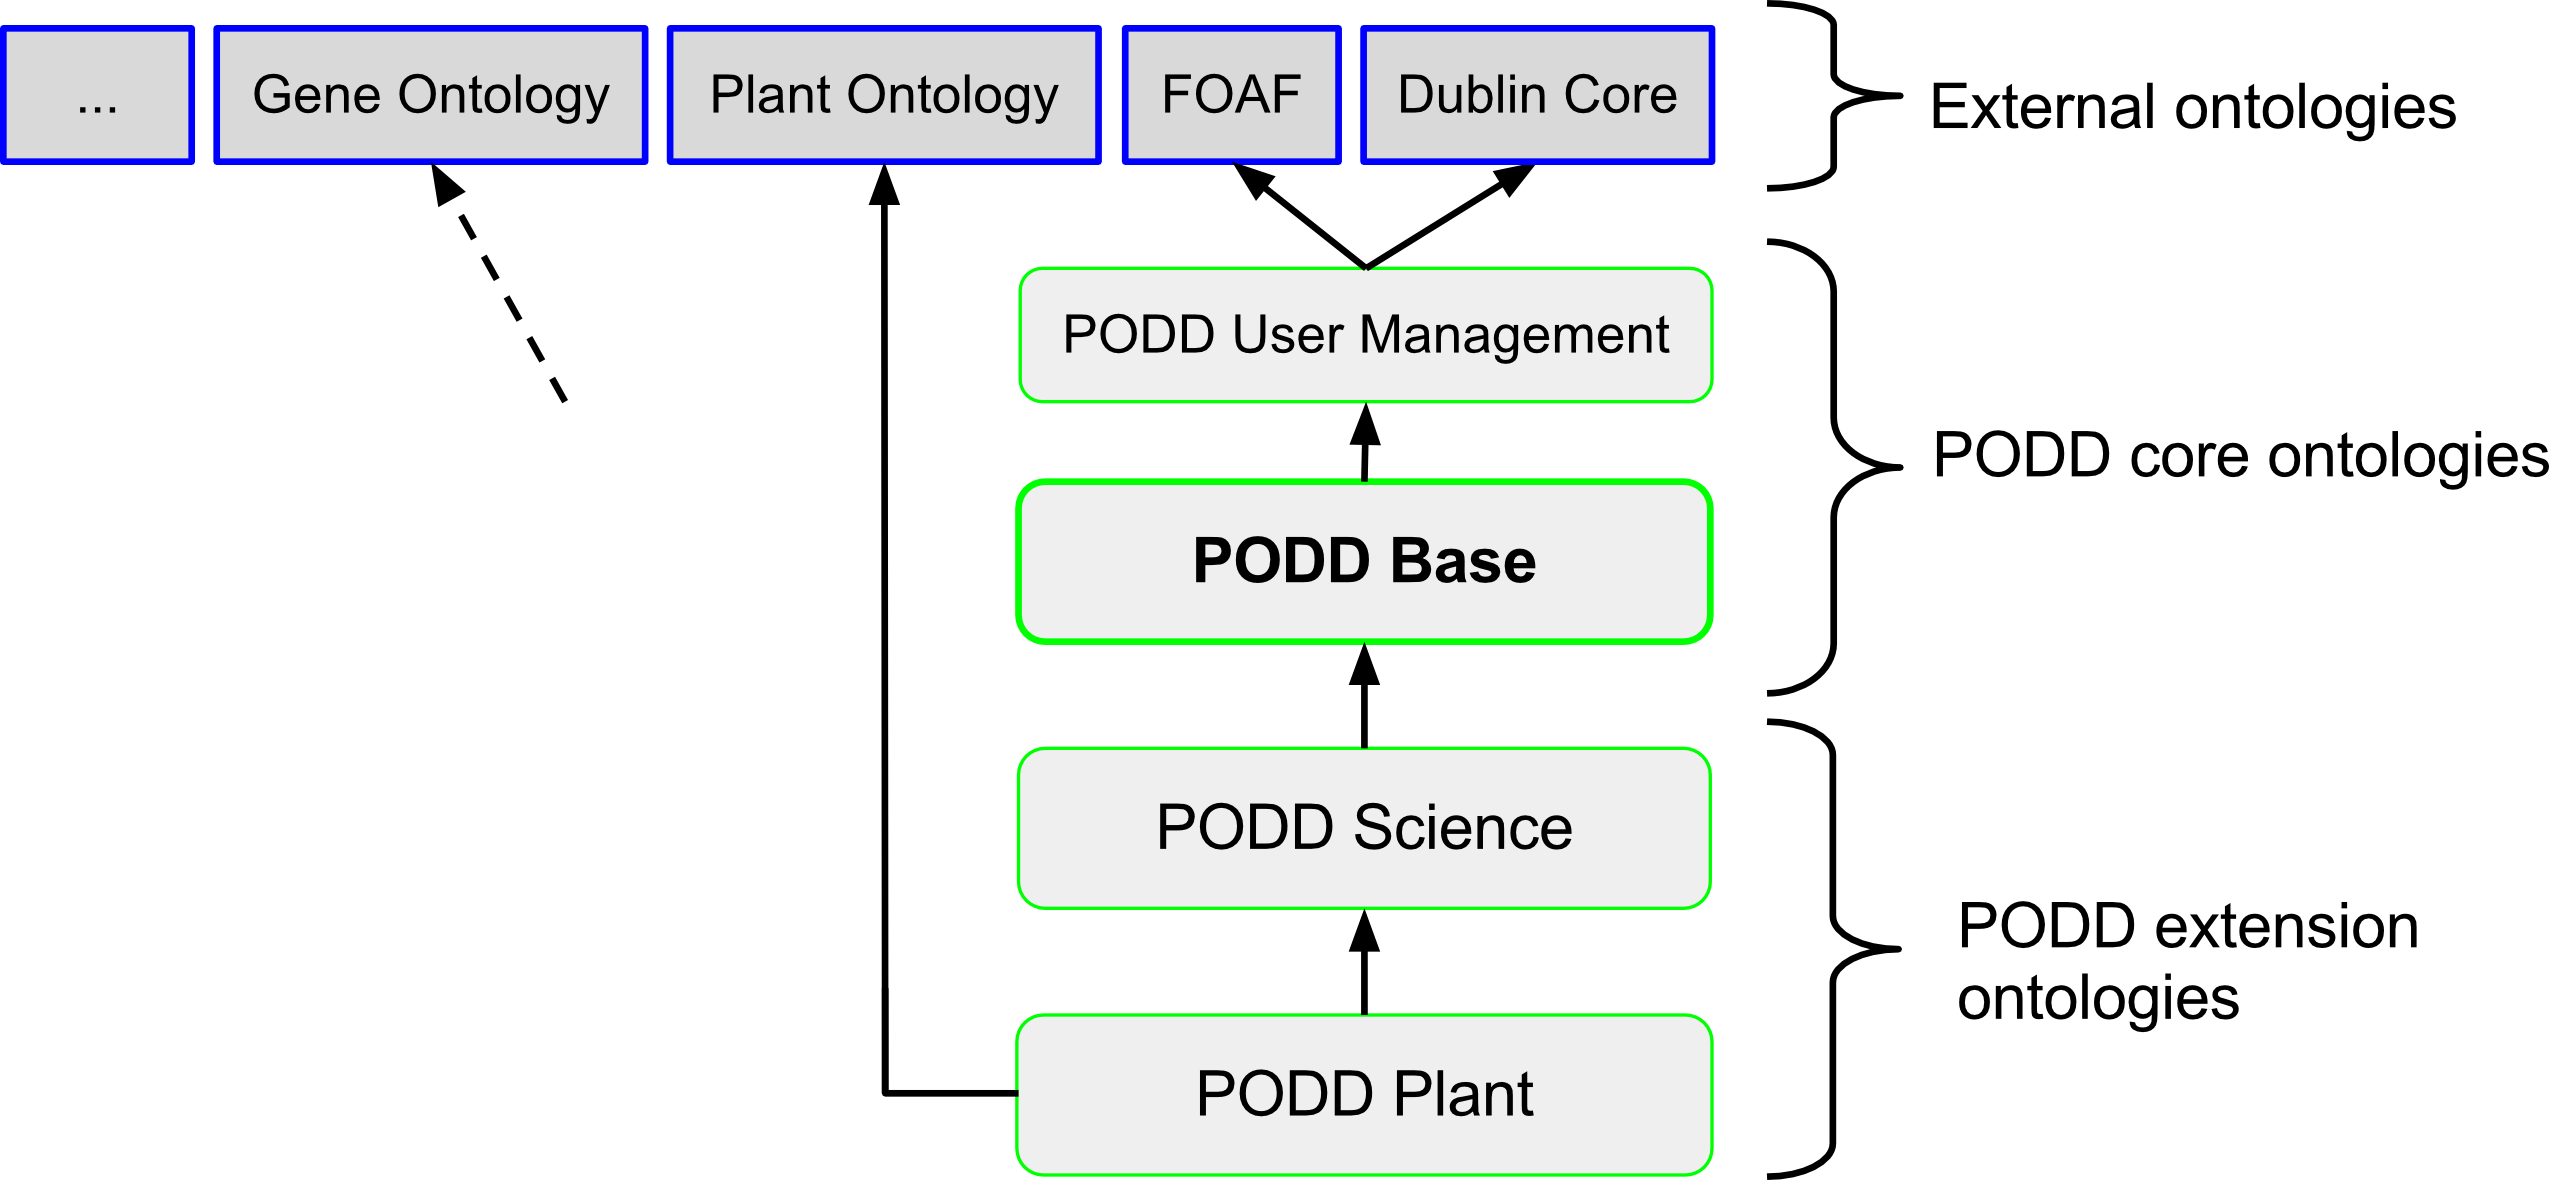
\includegraphics[width=12cm,keepaspectratio=true]{podd-ontologies-figure2.png}
 % podd-ontologies-figure2.png: 5097x2360 pixel, 600dpi, 21.58x9.99 cm, bb=0 0
%612 283

\caption{PODD ontology hierarchy}
\label{poddontologies}
\end{center}
\end{figure}


% An ontology is a common controlled vocabulary about a particular topic, in this
% case plant phenomics. The PODD Plant ontology therefore becomes an ontology for
% plant phenomics that extends the generally applicable PODD Science ontology with
% plant phenomics specific details \cite{Li2010}. This approach allows PODD to model
% multiple phenomics processes without enforcing a rigid data structure on
% objects, either now, in the past, or in the future. In addition, other community
% ontologies, such as the plant and gene ontologies \cite{Ashburner2000,Avraham2008}, can be used to
% annotate the data. This not only supports data discovery, but provides common
% reference points through which PODD managed data can be integrated with data in
% other research databases.


% The PODD application handles the instantiation and validation of objects based
% on the versions of ontologies that are specified by the user as being relevant.
% This gives PODD a unique extensibility as the domain knowledge is entirely
% captured in the ontology, and the operational aspects of the system are derived
% purely from the content of the ontology. In particular, PODD is designed around
% the ability to support multiple versions of ontologies concurrently. Previously
% published artifacts can be loaded without modification into PODD without
% affecting current studies that may be using newer, incompatible, versions of the
% schema ontologies.


% PODD is able to manage high volume, high resolution, heterogeneous datasets
% using a tree based structure, which in the PODD Science ontology is based on the
% concept of a ``Project''. 
% %(http://podd.plantphenomics.org.au/podd/). 
% Data
% references are inserted into projects using subproperties of the PODD
% ``contains'' predicate. When results are available they are inserted
% independently and cross-referenced with the data that they were derived from
% using a subproperty of the PODD ``refers to'' property. Each of the
% subproperties have constraints on the types of objects that are valid as sources
% and destinations, making it easy to both validate existing uses, and suggest
% potential targets based on a source and a property.


% The genotype of the plant alone does not determine the phenotype; it is the
% combination of the organism’s genome with the environmental conditions that
% determine the phenotype. PODD captures metadata on the genotype of the
% organism(s) under investigation. PODD also gathers comprehensive metadata on the
% environmental conditions and treatments that the biological samples are exposed
% to. This structure makes PODD suitable to queries by web agents thus  linking
% information contained in other data repositories, e.g genomics, transcriptomics,
% metabolomics to phenomics information.  

\section{CSIRO Data Access Portal}
CSIRO's Research Data Service (RDS) has developed the Data Access Portal (DAP),
an open source web application that enables research data to be discovered,
managed and shared. \cite{DAP}

Researchers can describe a data collection, deposit data, choose a license, and
add attribution details. Access to a collection's description and/or data can be
restricted to CSIRO or a set of individuals (within CSIRO or partner
organisations) or it can be made public, becoming searchable by anyone via the
Internet. In the case where a collection and its data are public, a Digital
Object Identifier (DOI) is issued and can be used to formally cite the
collection in a publication. 

%Collections can either be one-time, self-serve
%deposits or automated, ongoing deposits and can be changed over time through
%versioning. Whole datasets or specific files within a collection can be
%downloaded. A machine-to-machine REST interface permits programmatic search and
%collection download.


DAP is the visible part of the system. Other than standard web servers,
databases and application servers, additional required server-side
infrastructure includes petabyte-level, multi-decade, backed-up disk storage,
integrity checking, and automated migration of data collections to and from tape
storage.

\section{The PlantScan\textsuperscript{\texttrademark} digitisation platform}
% See unresolved comment at the end

%System description and Processes

\subsection{BagIt}

BagIt is defined by an Internet Engineering Task Force (IETF) document as an
``hierarchical file packaging format for storage and transfer of arbitrary
digital content''\cite{Kunze2011}. A payload manifest details content and MD5 or SHA hashes
for content integrity verification. Data file related metadata can be stored in
pre-defined files as key-value pairs. 

For PlantScan\textsuperscript{\texttrademark}, file-level metadata
includes plant barcodes, batch numbers, and plant type, although the BagIt
specification does not mandate a particular archiving strategy, with the
focus being upon the directory structure, special files, and integrity checking.
% Bag creation and payload manifest integrity checking, tools can take advantage
% of the multi-core capabilities of modern computing hardware. 
% To suit current
% needs, 
BagIt-conforming tools \cite{Summers} \cite{LoCBagger} were assessed and where necessary,
improvements were implemented and tested to ensure that the tools were fit for purpose in the CSIRO Advanced Scientific Computing (ASC) HPC environment.
% For example, the implementation of \cite{LoCBagger}
% assumed that as many threads as possible should be created for multi-threaded
% operations such as bag creation and payload manifest verification. On a HPC host
% with hundreds of processors, this can lead to runaway thread creation, so this
% needed to be addressed. Neither \cite{Summers} nor \cite{LoCBagger} permitted payload files in a bag to
% be listed. This has since been added to \cite{LoCBagger}. 
%Some functionality (not discussed
%here) present in [8] but not in \cite{Summers} was added to the latter.

\subsection{Bag preparation for a DAP collection}


CSIRO ASC shared facilities \cite{ASC} are used to process the raw
PlantScan\textsuperscript{\texttrademark} data to derive data products (meshes).
Raw data and meshes are collected using the BagIt format \cite{Kunze2011} and
stored in the ASC archival system. ASC High Performance Compute (HPC) hosts
(systems with high processor count and large memory) are taken advantage of to
create and verify bags more rapidly than would be possible on conventional
computer systems. 
CSIRO's HRPPC makes use of DAP to store collections of PlantScan\textsuperscript{\texttrademark} raw images and processed mesh data as bags.
%DAP is used to store collections of
%PlantScan\textsuperscript{\texttrademark} 
%raw images and processed mesh data as bags. 
Currently, one bag is equivalent to
a single batch scanned on the
PlantScan\textsuperscript{\texttrademark}
local software system, which usually means the same kind of plant with different
genotypes scanned under one  experiment configuration profile.  


Raw data from
PlantScan\textsuperscript{\texttrademark} 
local storage (HRPPC-Store) and data processed on HPC hosts are transferred to
ASC bulk storage where image and mesh files are organised in folders by batch,
then barcode number, then subfolders for each image file type, including RGB images,
IR images, and LiDAR (Light Detection and
Ranging Sensors, and their related meshes. Bag creation is carried out via an allocated ASC HPC job.
% However the
% naming, content and amount of data in a bag are flexible and depend upon the
% intention of the bag. For example, multiple batches can be packed into one bag
% when the batches come from one plant’s scans at different time points. The
% multi-threaded BagIt tool is called on the ASC HPC host to create a bag that is
% then compressed into a single file containing a top-level data folder, a
% manifest file that contains checksums for every data file, and tag files that
% contain the metadata description of the bag just packed. 
The metadata required for a DAP publication is created and the bag transferred
to the DAP staging area via SFTP (SSH File Transfer Protocol). After publication
of the DAP collection, the data from PlantScan\textsuperscript{\texttrademark}
for the given project becomes
discoverable via DAP. In addition, experiment reports, published papers, and
sensor configurations can either be made accessible via a DAP collection's
``related materials'' links, other metadata fields, or within the collection's
data (e.g. bag).

\subsection{Heterogeneous data streams}

PlantScan\textsuperscript{\texttrademark} is a medium throughput high resolution
phenotyping platform, which brings together a number of imaging sensors--light 
detection and ranging, far-infrared imaging, and multi-wavelength imaging--to non-invasively measure plant growth and function using in-silico approaches.
% FIXME: TODO: [REF?] for PlantScan. 
Raw data is captured with
its contextual information (e.g. system configuration, time of acquisition,
batch number and project) and is stored in a purpose-built database as the data
is being generated. The various data streams are collated and used to produce
full 3D representation of each plant with overlaid spectral information. The
metadata collected during image acquisition are necessary inputs for the
computer vision techniques which are used to create the 3D representation of the
plant.
% FIXME: TODO: Create Figure 3
%(Figure 3)[e]. 
The 3D meshes are then automatically segmented in order to
semantically identify the different parts of the plants (Paproki et al, 2012). A
longitudinal 3D matching pipeline for plant mesh parts is then used to evaluate 
temporal changes at the whole plant and/or organ level. 

% After initial processing to recreate the 3D structure, the raw data for each plant is packaged into
% one location using BagIt. All bags belonging to the
% same specific PODD project are grouped into collections on the CSIRO Data Access
% Portal. These bags have a permanent address which is recorded into PODD. Any
% additional processes on these digital objects (such as statistical information
% on features like plant colour, volume,  growth etc. and on elements such as
% petiole, stem, leaf) are also captured by PODD using the properties in the 
% PODD Plant Ontology (Figure~\ref{poddontologies}).

\subsection{Metadata}
Each acquisition on PlantScan\textsuperscript{\texttrademark} includes metadata
(in addition to the raw data
streams), such as plant genus and species, project and experiment metadata, a
unique identifier for each image (Globally Unique Identifier), imaging angle,
environmental temperature of the imaging chamber, location of optical and colour
calibration datasets for each acquisition run, and LiDAR calibration files. The metadata associated with each
acquisition is automatically generated when setting up the configuration on the
platform. This information is paramount to validate and process the raw image
data, and for the post-processing phases. 
% This information currently resides in
% the PlantScan\textsuperscript{\texttrademark} database.


\subsection{Data volume}
Digitisation systems such as PlantScan\textsuperscript{\texttrademark} generate
huge amounts of data including
raw image data, registration metadata, sensor configurations and plant metadata.
For example, PlantScan\textsuperscript{\texttrademark} generates around 500GB of
raw image data, representing
in excess of 200,000 database records, per day. Sufficient storage space
(usually at remote locations) and fast network transfer rates are thus
necessary to facilitate data movement for processing using high performance
computers (HPC). Because an RDF database structure is not suitable for handling
large data sets of images, it is necessary to package the raw information into
elementary units with permanent addresses which could be retrieved using PODD. 
The CSIRO DAP \cite{DAP} and ASC storage and compute facilities \cite{ASC} are key
resources used by PlantScan\textsuperscript{\texttrademark} to
process and store bulk data.


\section{Semantic integration}
The PODD ontology enables plant phenomics researchers to link from mesh results
to the raw data that they were generated from. It also allows researchers to
link from both mesh results and their recorded conclusions to shared phenomics
ontologies which describe specific features of the plants. When used together,
this enables scientists to trace the provenance of their results and conclusions
based on well known concepts in phenomics ontologies.


% The PODD ontology allows sparse annotation of data and results, so scientists
% are not required to annotate all of their data with links to shared ontologies
% by default. However, the system is extensible, so in future such a requirement
% could be added in a new version of the PODD ontology while maintaining backwards
% compatibility with previous experiments that may be published or immutable.


External ontologies must currently be mapped into the PODD system to define the
expected status of the classes and properties with respect to the basic PODD
concepts. The basic concepts are used to both verify that each PODD project has
a single valid tree structure, and render HTML pages for both browsing and
editing. PODD also supports an RDF-based HTTP REST interface that clients may
use to fetch and update objects without using the HTML pages.


\section{Semantic publication}
PODD provides a secure mechanism for publishing both human and machine readable
descriptions of scientific experiments. It utilises the well-known DOI mechanism
for publishing raw data files using DAP, and uses HTTP URIs to publish
experiments using the PODD web interface.


% PODD implements support for Content Negotiation, with common RDF serialisations
% supported in addition to HTML pages that are encoded with RDFa (RDF in
% Attributes). Although most non-human agents will receive an RDF formatted
% document when they resolve a PODD URI, if a PODD HTML page is saved the
% annotations can still be retrieved using RDFa. 


Scientific journals increasingly require the data and provenance for articles to
be available in a machine readable format. The DOI registrar that DAP uses,
DataCite \cite{Brase2009}, was setup to provide unique identifiers for data
items that can
be attached to publications, which in turn may have their own DOIs.


By providing machine readable descriptions of scientific experiments, including
semantic references to shared ontologies where possible, PODD enables the output
from PlantScan\textsuperscript{\texttrademark} to be interpreted and extended by
others. The use of PODD URIs
in other RDF documents enables scientists to extend the initial work using the
Linked Data paradigm \cite{BernersLee}.


\section{Conclusion}
This paper described how the Phenomics Ontology Driven Data repository
integrates with the PlantScan\textsuperscript{\texttrademark} platform and CSIRO
Data Access Portal to manage
the complex workflows at the High Resolution Plant Phenomics Centre. This
workflow keeps track of phenomics data, metadata and experimental processes and
also provides a secure mechanism to share and publish scientific experiments in
both human and machine readable formats.

\bibliographystyle{splncs}
\bibliography{podd-bibliography}

%References
%[1] http://www.iucr.org/\_\_data/iucr/lists/epc-l/pdf00003.pdf
%[2] http://topbraid.org/spin/api/
%[3] http://www.plantontology.org/
%[4] http://www.geneontology.org/
%[5] https://wiki.csiro.au/confluence/display/dmsdoc/Home
%[6] http://datatracker.ietf.org/doc/draft-kunze-bagit/
%[7] https://pypi.python.org/pypi/bagit/
%[8] http://sourceforge.net/projects/loc-xferutils/
%[9] http://sourceforge.net/projects/loc-xferutils/files/loc-bagger/
%[10] https://wiki.csiro.au/display/ASC
%[11] doi:10.1109/COINFO.2009.66 
%[12] doi:10.1016/j.jbi.2008.03.004
%[13] doi:10.1007/978-3-642-13654-2\_22
%[14] http://www.w3.org/DesignIssues/LinkedData.html

\end{document}
% Unresolved comments from Google docs:
%
% [a]Xavier Sirault:
% NOTE:Submitted papers should not exceed 15 pages for long papers and 8 pages
%for
% short papers and must be formatted according to the LNCS guidelines. 
%  
% Proceedings of the workshop will be published online at CEUR Workshop
% Proceedings (www.CEUR-WS.org ). The 3 best papers presented at the workshop
%will
% be included in the supplementary Springer LNCS (Lecture Notes in Computer
% Science ) proceedings of the ESWC2013 conference.
% ________________
% ansell.peter:
% I will reformat the document tommorrow morning using Latex and distribute the
% PDF to others for a final check.
% [b]Xavier Sirault:
% currently 78 words
% ________________
% Xavier Sirault:
% now 126 words
% ________________
% Xavier Sirault:
% 136 words
% [c]David Benn:
% "DAP" has been removed from the abstract. I know it looms large in the paper
%but
% is it worth adding something like "and data collection publication"? I've
%added
% this in but I understand if it's not okay because we're space challenged.
% ________________
% Xavier Sirault:
% No worries, I think the paper reads quite well. I would look at it tomorrow
% again
% ________________
% Xavier Sirault:
% to try to link some loose ends
% ________________
% David Benn:
% Okay, good. I'll do the same.
% ________________
% David Benn:
% I've read through, made suggestions for correction, chatted with Peter about
% them. I'll check back later tonight.
% [d]Xavier Sirault:
% I do not like this title. I do not want the paper to describe plantscan per se
% but more the acquisition processes and how it is captured.
% ________________
% David Benn:
% How about something like: "Plant phenomics imaging, processing, metadata
%capture
% and publication". Too verbose I know.
% [e]Xavier Sirault:
% Jianming, could you please put a 3D model of tobacco with overlaid RGB signal?
% [f]Xavier Sirault:
% This figure is figure 1. I think we should put it there rather than at the end
% of the introduction
% ________________
% David Benn:
% Do we want to simply change "Figure 4" to "Figure 1" here, or are you
%suggesting
% we move the diagram?
% ________________
% David Benn:
% Looks like this has been resolved.
% ________________
% David Benn:
% Not sure whether this is all we want to do or to physically move Fig 1 to
%here.
